\section{Performance analyse} \label{sec:performance}

Tijdens de ontwikkeling van de library is duidelijk geworden dat de performance van de geschreven programma's niet altijd optimaal is. Met name bij programma's die gebruik maken van \emph{timers} en bij programma's met een uitgebreide grafische boom.

Dit performance probleem kan twee oorzaken hebben, ten eerste is het mogelijk dat de module van de applicatie niet snel genoeg JSON-berichten kan coderen en anderzijds is het mogelijk dat de client de binnengekomen berichten niet snel genoeg kan verwerken.

Eerst is gekeken naar de performance van de module, hiervoor is voornamelijk gekeken naar het geheugengebruik gezien er het vermoeden was dat de module mogelijk te veel geheugen zou gebruiken (mogelijk door een geheugenlek) en voortdurend bezig is met garbage collection. Na een heap profile gemaakt te hebben bleek dat de Haskell code in totaal 600kb aan geheugen gebruikt, en dit getal stabiel is. Hieruit blijkt dat het probleem niet in de module zit.

\subsection{Performance JavaScript-code}

De analyse van de client van Canvas.hs brengt een groter probleem aan het licht. In het ontwerp is ervoor gekozen de grafische boom stateless te maken. Dit betekend dat, zodra een nieuwe tekenactie door de module vertaald wordt, de client de hele grafische boom opnieuw doorgestuurd krijgt. In de client wordt deze grafische boom volledig opnieuw getekend. Hiervoor dient onder andere eerst een nieuwe \emph{stage} opgebouwd te worden.
Het opbouwen van de stage bleek erg kostbaar te zijn en duurde KineticJS ongeveer 6 ms (tegen 0.5 ms voor het opnieuw tekenen van dezelfde stage). Dit hebben is gemeten met de JavaScript-profiler in Google Chrome. De exacte getallen zijn niet direct interessant bij een CPU-profiel, de verhouding daarentegen wel. Het feit dat het opbouwen van de stage twaalf maal langer duurt dan het tekenen van het test programma bevestigd het probleem.

In \autoref{sec:aanbevelingen} wordt een aanbeveling gedaan voor het aanpakken van dit performance probleem. Hierin wordt voorgesteld updates incrementeel uit te laten voeren waarbij niet bij elk bericht van de module de stage opnieuw opgebouwd hoeft te worden. Om dit te realiseren zal wel een groot deel van de code en hoogstwaarschijnlijk ook de API aangepast moeten worden.

\subsection{Performance Haskell-code}

In de module is een optimalisatie doorgevoerd die te maken heeft met het vertalen van strings naar verschillend types. Er was het vermoeden dat er in de Haskell-code van Canvas.hs veel performance verloren zou gaan doordat we \inlinecode{Strings} naar \inlinecode{ByteStrings} naar \inlinecode{Text} vertaalde. Het bleek dat de laatste vertaalslag overbodig is, en daarom is deze verwijderd. Hieronder volgen twee grafieken, \autoref{fig:performance1} en \autoref{fig:performance2}~, die het geheugengebruik van de module van Canvas.hs demonstreren met en zonder de extra translaties.

Uiteindelijk blijkt deze wijziging weinig verschil gemaakt te hebben in het totale geheugengebruik. Desondanks was de optimalisatie niet voor niets gezien het de Haskell-code een stuk leesbaarder heeft gemaakt. Wel is te zien dat in het eerste figuur de garbage collecting van Haskell agressiever lijkt, dus wellicht wordt zonder de wijziging toch meer memory tijdelijk gebruikt en vervolgens direct weer vrijgegeven. Verder valt op dat na de optimalisatie er toch \inlinecode{Text} in de heap profile staat. Dit is vermoedelijk omdat een van de libraries die gebruikt wordt door Canvas.hs daar intern gebruik van maakt.

Voor dit specifieke geval zijn de heap profiles niet interessant, het grootste gedeelte van de data is \emph{PINNED} data, dit zijn vooral \inlinecode{ByteString} allocaties. Gezien de module vooral een translator is van het protocol naar een aantal \inlinecode{ByteStrings} is dit niet verrassend. Wel bieden dit soort grafieken duidelijk inzicht in of er geheugenlekken zijn en of er onnodige conversies gemaakt worden, voor grote projecten zijn dit soort grafiekjes zeker nuttig.

\begin{figure}[H]
\begin{center}
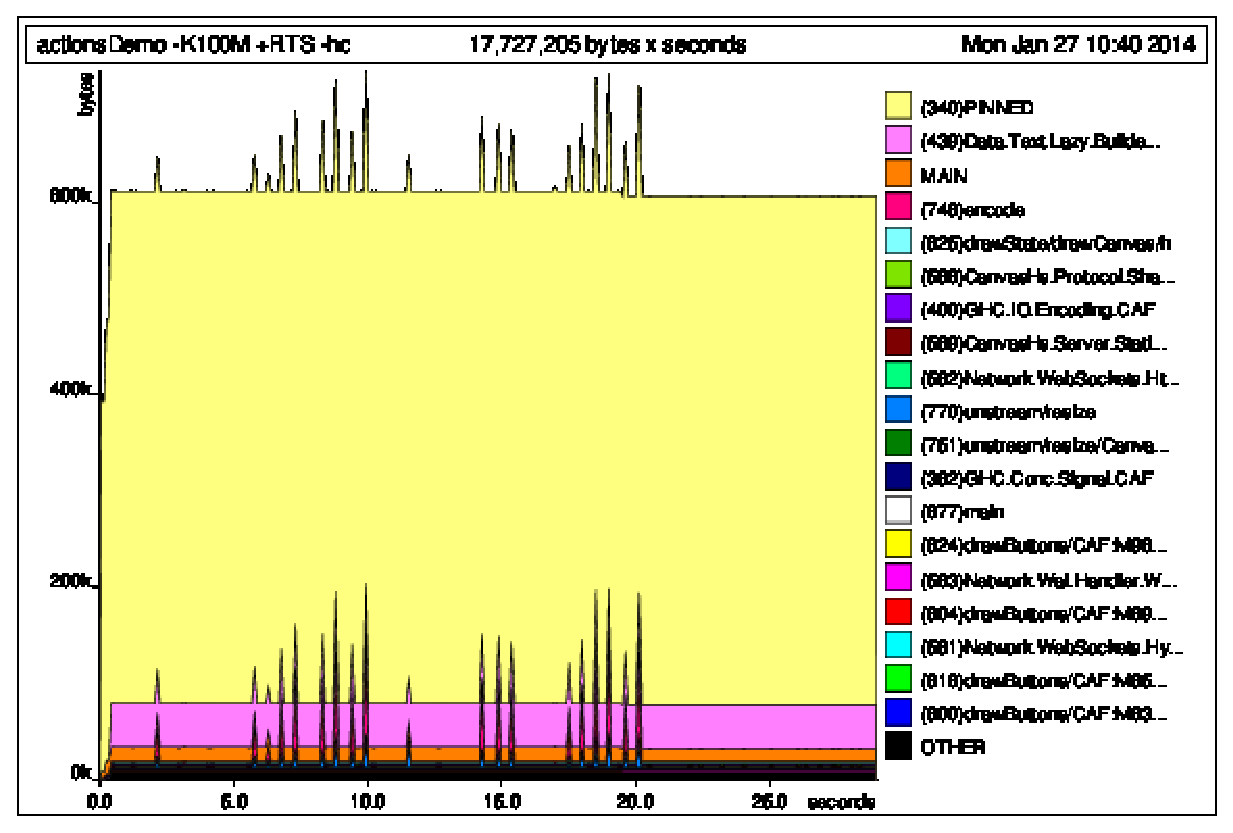
\includegraphics[keepaspectratio,width=0.8\textwidth]{./images/actionsDemoBeforeByteStrings.eps}
\caption{Heap profile voor de wijziging}
\label{fig:performance1}
\end{center}
\end{figure}

\begin{figure}[H]
\begin{center}
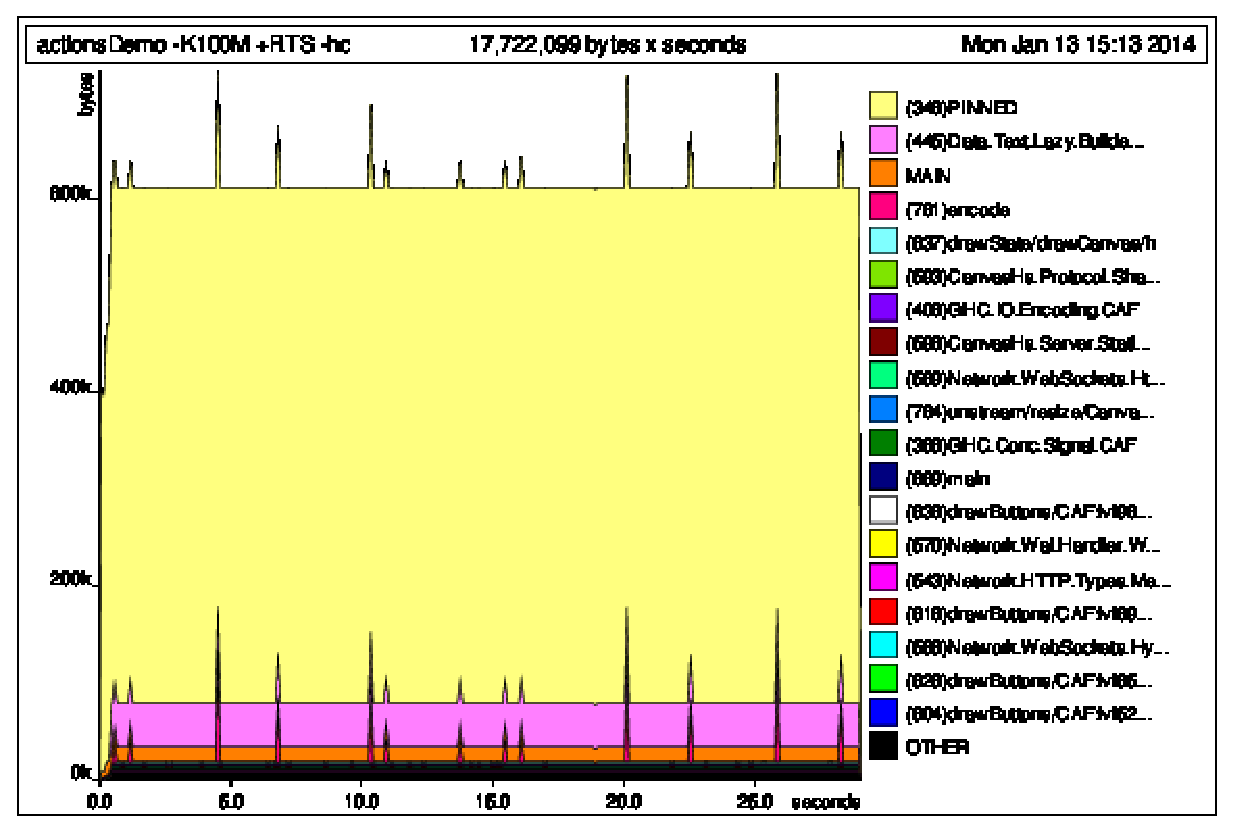
\includegraphics[keepaspectratio,width=0.8\textwidth]{./images/actionsDemoAfterByteStrings.eps}
\caption{Heap profile na de wijziging}
\label{fig:performance2}
\end{center}
\end{figure}
